\documentclass{article}
\title{Comparing estimation results from GeoDaSpace, Stata and R: reasons for difference and pathway for matching}
\author{}
\usepackage{amsmath}
\usepackage{natbib}
\bibpunct{(}{)}{,}{a}{}{,}
\usepackage{float}
\usepackage{xcolor}
\usepackage{listings}
\usepackage{caption}
\usepackage{hyperref}
\usepackage{subfig}
\usepackage{color,soul}
\usepackage[section]{placeins}
\usepackage{graphicx}
\graphicspath{{figures/}}
\DeclareCaptionFont{white}{\color{white}}
\DeclareCaptionFormat{listing}{%
  \parbox{\textwidth}{\colorbox{gray}{\parbox{\textwidth}{#1#2#3}}\vskip-4pt}}
\captionsetup[lstlisting]{format=listing,labelfont=white,textfont=white}
\lstset{frame=lrb,xleftmargin=\fboxsep,xrightmargin=-\fboxsep}
\newfloat{code}{H}{myc}

\begin{document}
\maketitle
\section{Introduction}
In this document we compare the results of models with spatial error from 3 different programs: GeoDaSpace, R and Stata. Despite all the methods available in GeoDaSpace, here we show only those which yield discrepant results in GeoDaSpace in comparison with Stata. An explanation for the differences is provided. In addition, we show how to set the preferences in GeoDaSpace in order to get the same results from Stata. When this option is not available, we show how PySAL, a Python library on which GeoDaSpace is based, can be used to match Stata.

The following spatial error models (SEM) are discussed in this document:

\begin{itemize}
\item SEM with exogenous variables and no heteroskedasticity
\item SEM with endogenous variables and no heteroskedasticity
\item SEM with spatial lag and no heteroskedasticity
\item SEM with exogenous variables and heteroskedasticity
\item SEM with endogenous variables and heteroskedasticity
\item SEM with spatial lag and heteroskedasticity
\end{itemize}

\section{Spatial Error Models without Heteroskedasticity}

To estimate the spatial error model without heteroskedasticity (the K-P-D model) in GeoDaSpace, we need only to check the box ``Spatial Error", as shown in Figure \ref{f:GS_hom}. Given the particular specification of the model since all variables as exogenous, as presented in \citet{Anselin11}, the results from GeoDaSpace do not match those from Stata or the package sphet in R. This discrepancy is due to an error in Stata for the case of a spatial error model with exogenous variables only. In Stata, the exogeneity is ignored and a two-stage least squares estimation is performed instead of the OLS. Table \ref{t:res_hom} compares the results from GeoDaSpace, Stata and R (package sphet). The K-P-D method is not available in the released version of sphet (v. 1.1-12, published on CRAN on 2012-04-13). In this document, we call this version sphet1. Nonetheless, the results presented here can be obtained using the alpha version from R-Forge, revision 56, published on 2012-07-22. This newer version of the code is henceforth referred as sphet2\footnote{Given that it is an alpha version, the code is subject to change.}. when only exogenous variables are considered. The results from GeoDaSpace are also different than sphet's. 

\begin{figure}[htb]
\caption{Estimation of spatial error models using GeoDaSpace}
\label{f:GS_hom}
\begin{center}
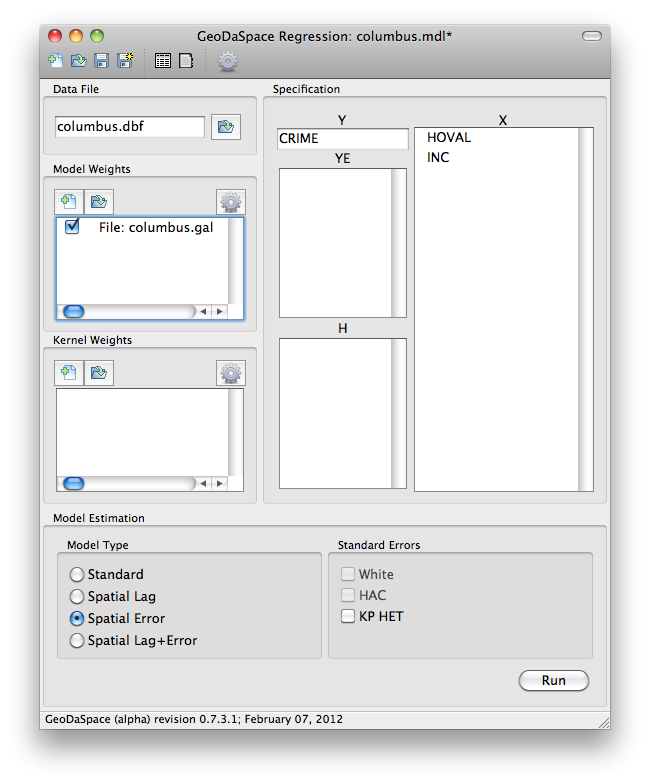
\includegraphics[width=0.7\linewidth]{GS_hom.png}\\
%\scriptsize{}
\end{center}
\end{figure}

\begin{table}[htpb]
\caption{Comparison of the results of spatial error models with exogenous variables and no heteroskedasticity}
\label{t:res_hom}
\centering
\begin{small}
\begin{tabular}{l|cccc} \hline
\textbf{Variable}&\textbf{GeoDaSpace}&\textbf{sphet2}&\textbf{Stata}&\textbf{PySAL$^1$}\\ \hline
CONSTANT&8.0259&6.6762&6.9884&6.9884\\
&(0.3601)&(0.3498)&(0.3605)&(0.3605)\\
RD90&4.3228&3.9450&3.9945&3.9945\\
&(0.1596)&(0.1553)&(0.1612)&(0.1612)\\
UE90&-0.2753&-0.0770&-0.1240&-0.1240\\
&(0.0479)&(0.0471)&(0.0490)&(0.0490)\\
lambda&0.4572&0.4149&0.4124&0.4124\\
&(0.0189)&(0.0194)&(0.0194)&(0.0194)\\
\hline
\multicolumn{5}{l}{\scriptsize{$^1$PySAL using the code to match Stata as in Listing \ref{lt:hom_stata}.}} \\
\end{tabular}
\end{small}
\end{table}


Despite the problems with Stata's estimator, PySAL allows us to match its results. To do so, we have to use PySAL's Base classes, that allows us to specify the model more freely. Since Stata performs a 2SLS estimation, in order to match its results using PySAL we have to specify X as both the endogenous variables and the instruments. Since PySAL requires at least one exogenous variable, we create a constant to use as such. In addition to the different treatment given to exogenous variables in Stata, the A1 matrix used to estimate the model is also different. In GeoDaSpace's code, the option was for the use of the matrix proposed by \citet{Arraiz10} instead of \citet{Drukker10} and \citet{Drukker11}. The details of this choice can be found in \citet{Anselin11}. Listing \ref{lt:hom_stata} shows the command that will allow PySAL to match the results from Stata for the spatial error model\footnote{A walkthrough for the estimation of spatial error models without heteroskedasticity using PySAL can be found at \url{http://pysal.geodacenter.org/dev/library/spreg/error_sp_hom.html}}. 

\begin{code}
\begin{lstlisting}[label=lt:hom_stata,caption=Using PySAL to match the results of spatial error models from Stata,language=Python]

import pysal
import numpy as np

w = pysal.open('NAT_queen.gal').read()
w.transform = 'r'
db = pysal.open('NAT.dbf')
hr90 = np.array([db.by_col('HR90')]).T
rd90 = np.array([db.by_col('RD90')]).T
ue90 = np.array([db.by_col('UE90')]).T

ones = np.ones(crime.shape)
model = pysal.spreg.BaseGM_Endog_Error_Hom(hr90, ones,
        yend=x, q=x, w=w, A1='hom_sc')

print model.betas
print map(np.sqrt, model.vm.diagonal())

\end{lstlisting}
\end{code}

If we have endogenous variables, or a spatial lag, the problem in Stata's code no longer exists, since we now do have to run a 2SLS estimator. Nonetheless, the results from GeoDaSpace remain different from those from Stata and R, as shown in Table \ref{t:res_hom_endog}. The diffence is due to the choice of the A1 matrix used in the estimations and, for the spatial lag, the number of lags of the exogenous variables used as instruments. Figure \ref{f:GS_hom_endog} shows how to estimate the spatial error model with endogenous variables or with a spatial lag. Of course, the combination of the two, i.e. spaital lag and other endogenous variables, is also possible.

\begin{figure}[htb]
\centering
\caption{Estimation of spatial error models with endogenous variables or spatial lag using GeoDaSpace}
\label{f:GS_hom_endog}
\subfloat[Spatial error with endogenous variable]{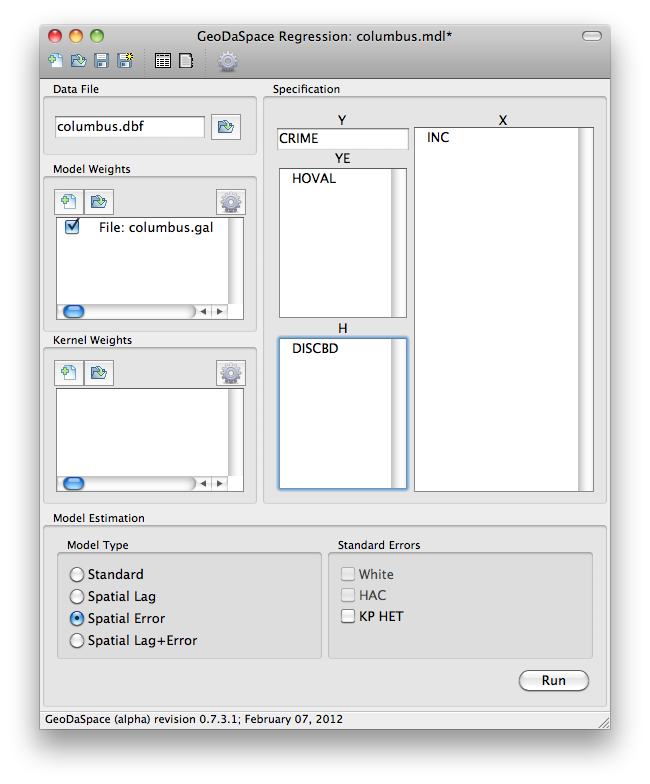
\includegraphics[width=0.5\textwidth]{GS_hom_endog.png}}
\subfloat[Spatial error and lag]{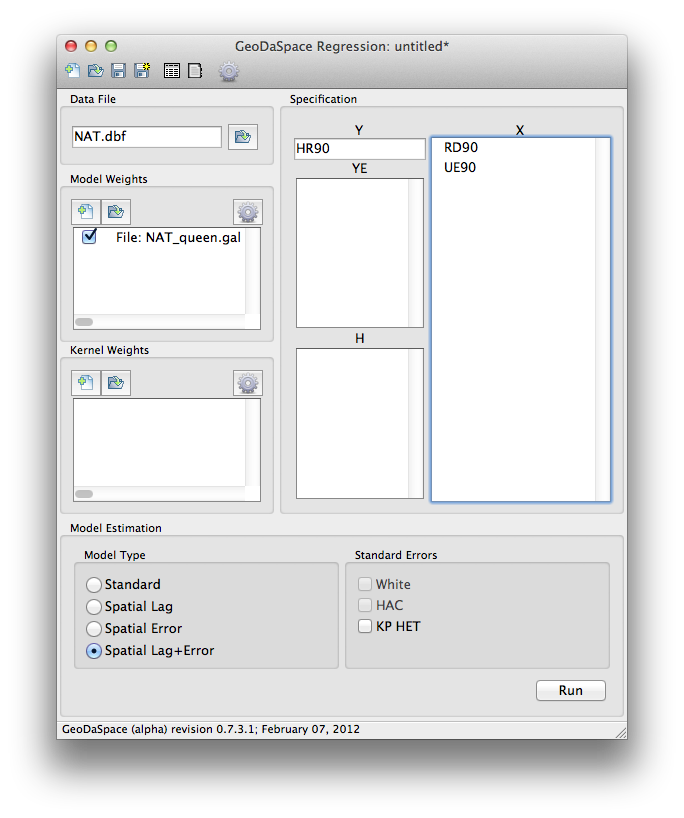
\includegraphics[width=0.5\textwidth]{GS_hom_combo.png}} \\
\end{figure}

\begin{table}[htpb]
\caption{Comparison of the results of spatial error models with endogenous variables or spatial lag}
\label{t:res_hom_endog}
\centering
\begin{small}
\begin{tabular}{l|cccc} \hline
\multicolumn{5}{c}{\textbf{Spatial error with HOVAL as endogenous variable}} \\ \hline
\textbf{Variable}&\textbf{GeoDaSpace}&\textbf{sphet2}&\textbf{Stata}&\textbf{PySAL$^1$}\\ \hline
CONSTANT&82.2068&&82.5747&\\
&(16.3992)&&(16.3797)&\\
INC&0.5785&&0.5810&\\
&(1.3543)&&(1.3606)&\\
HOVAL$^2$&-1.4374&&-1.4481&\\
&(0.7904)&&(0.7925)&\\
lambda&0.3910&&0.3765&\\
&(0.1962)&&(0.1921)&\\
\hline
\multicolumn{5}{c}{\textbf{Spatial error with spatial lag}} \\ \hline
\textbf{Variable}&\textbf{GeoDaSpace$^3$}&\textbf{sphet2}&\textbf{Stata}&\textbf{PySAL$^1$}\\ \hline
CONSTANT&6.9406&6.9362&6.9362&6.9362\\
&(0.5327)&(0.5120)&(0.5120)&(0.5120)\\
RD90&4.0074&4.0061&4.0061&4.0061\\
&(0.1758)&(0.1764)&(0.1764)&(0.1764)\\
UE90&-0.0957&-0.0978&-0.0978&-0.0978\\
&(0.0490)&(0.0481)&(0.0481)&(0.0481)\\
W\_HR90&-0.0220&-0.0190&-0.0190&-0.0190\\
&(0.0543)&(0.0513)&(0.0513)&(0.0513)\\
lambda&0.5098&0.4364&0.4364&0.4364\\
&(0.0376)&(0.0421)&(0.0421)&(0.0421)\\
\hline
\multicolumn{5}{l}{\scriptsize{$^1$PySAL using the code to match Stata as in Listing \ref{lt:hom_end_stata}.}} \\
\multicolumn{5}{l}{\scriptsize{$^2$DISCBD is used to instrument HOVAL.}} \\
\multicolumn{5}{l}{\scriptsize{$^3$GeoDaSpace using 2 spatial lags for the instruments.}} \\
\end{tabular}
\end{small}
\end{table}

Once again, PySAL offers the possibility of matching Stata. As shown in Listing \ref{lt:hom_end_stata}, all that we have to do is to select the option `hom\_sc' for the argument A1. By doing so, we override the default A1=`het', in which the matrix A1 is defined as in \citet{Arraiz10} by opting for the A1 as used in Stata and presented in \citet{Drukker10} and \citet{Drukker11}. For the case of a spatial lag, it is also important to set the amount of spatial lags of the exogenous variables to be used as instrument of the spatial lag of the dependent variable. The default used in GeoDaSpace is `1'. The value must be changed to `2' in order to match Stata's results. The code shown in Listing \ref{lt:hom_end_stata} continues from Listing \ref{lt:hom_stata}.

\begin{code}
\begin{lstlisting}[label=lt:hom_end_stata,caption=Using PySAL to match the results of spatial error models with endogenous variables or spatial lag from Stata,language=Python]

#Spatial error model with spatial lag:
model = pysal.spreg.GM_Combo_Hom(hr90, np.hstack((rd90,
        ue90)), w=w, A1='hom_sc', w_lags=2)
print model.summary

#Adding instrument 'FP89':
fp89 = np.array([db.by_col('FP89')]).T

#Spatial error model with UE90 as endogenous variable:
model = pysal.spreg.GM_Endog_Error_Hom(hr90, rd90,
        yend=ue90, q=fp89, w=w, A1='hom_sc')
print model.summary

\end{lstlisting}
\end{code}

\section{Spatial Error Models with Heteroskedasticity}
To estimate a spatial error model with heteroskedasticity in GeoDaSpace, we need to check the boxes "Spatial Error" for model type and `KP-Het' for standard errors, as shown in Figure \ref{f:GS_het}.

\begin{figure}[htb]
\caption{Estimation of spatial error models with heteroskedasticity using GeoDaSpace}
\label{f:GS_het}
\begin{center}
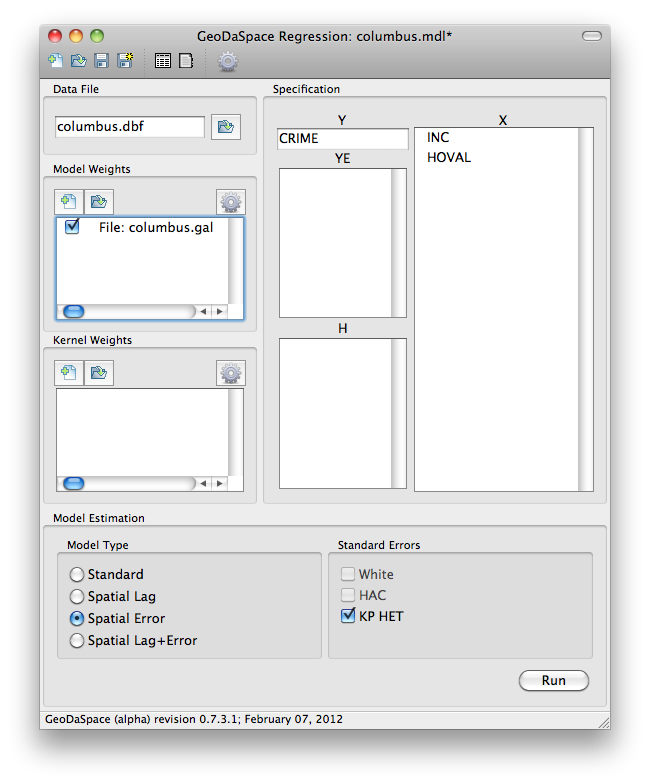
\includegraphics[width=0.7\linewidth]{GS_het.png}\\
%\scriptsize{}
\end{center}
\end{figure}

As in the case with no heteroskedasticity, Stata's code has an error in the estimation of the spatial error model with exogenous variables only. Therefore, it is not possible to match the results from Stata for this specification using GeoDaSpace. Table \ref{t:res_het} compares GeoDaSpace's results against Stata and the package sphet from R. As already stated, we refer to the released version 1.1-12 of sphet as sphet1 and the updated alpha version of spreg available from R-Forge (revision 56 published on 2012-07-22) is referred as sphet2. Differently than sphet2, the version sphet1 does not allow us to skip step1c in the estimation of the method. Please check Section \ref{s:step1c} for more details on this.

\begin{table}[htpb]
\caption{Comparison of the results of spatial error models with exogenous variables and heteroskedasticity}
\label{t:res_het}
\centering
\begin{small}
\begin{tabular}{l|ccccc} \hline
\textbf{Variable}&\textbf{GeoDaSpace}&\textbf{sphet1}&\textbf{sphet2}&\textbf{Stata}&\textbf{PySAL$^1$}\\ \hline
CONSTANT&6.6586&6.5782&6.6586&6.9777&6.9777\\
&(0.4749)&(0.4594)&(0.4745)&(0.4622)&(0.4622)\\
RD90&3.9417&3.9275&3.9417&3.9911&3.9911\\
&(0.2602)&(0.2316)&(0.2599)&(0.2326)&(0.2325)\\
UE90&-0.0745&-0.0630&-0.0745&-0.1225&-0.1225\\
&(0.0611)&(0.0589)&(0.0611)&(0.0592)&(0.0592)\\
lambda&0.4753&0.4756&0.4740&0.4721&0.4721\\
&(0.0235)&(0.0237)&(0.0237)&(0.0236)&(0.0236)\\
\hline
\multicolumn{6}{l}{\scriptsize{$^1$PySAL using the code to match Stata as in Listing \ref{lt:het_stata}.}} \\
\end{tabular}
\end{small}
\end{table}

In PySAL, it is possible to mimic the problem in Stata's code to estimate a model that yields the same results. The code is shown in Listing \ref{lt:het_stata}.

\begin{code}
\begin{lstlisting}[label=lt:het_stata,caption=Using PySAL to match the results of spatial error models with heteroskedasticity from Stata,language=Python]

import pysal
import numpy as np

w = pysal.open('NAT_queen.gal').read()
w.transform = 'r'
db = pysal.open('NAT.dbf')
hr90 = np.array([db.by_col('HR90')]).T
rd90 = np.array([db.by_col('RD90')]).T
ue90 = np.array([db.by_col('UE90')]).T

model = pysal.spreg.BaseGM_Endog_Error_Het(hr90, ones,
        yend=x, q=x, w=w)

print model.summary

\end{lstlisting}
\end{code}

When the spatial error model with heteroskedasticity contains a spatial lag, the default specification in GeoDaSpace does match the results from Stata. This is due to the order of the spatial lags of the exogenous variables used as instruments of the spatial lag of the dependent variable. The default in GeoDaSpace is a single lag. In Stata however the model is run lagging the exogenous variables twice. This option cannot be changed in Stata. In GeoDaSpace, we can choose the number of lags desired from the Preferences Panel. If we select `2' as the order of spatial lags for instruments, the results from GeoDaSpace match Stata's, as shown in Table \ref{t:res_het_combo}. Figure \ref{f:GS_het_combo} shows how to estimate a spatial error model with spatial lag and heteroskedasticity in GeoDaSpace, in addition to the preference panel where it is possible to define the order of the spatial lags for the instruments. The button that allows the access to the preference panel is highlighted in the figure.

\begin{table}[htpb]
\caption{Comparison of the results of spatial error models with spatial lag and heteroskedasticity}
\label{t:res_het_combo}
\centering
\begin{small}
\begin{tabular}{l|ccccc} \hline
\textbf{Variable}&\textbf{GeoDaSpace$^1$}&\textbf{sphet1}&\textbf{sphet2}&\textbf{Stata}&\textbf{PySAL$^2$}\\ \hline
CONSTANT&6.9406&7.0196&6.9406&6.9406&6.9406\\
&(0.8600)&(0.8251)&(0.8600)&(0.8600)&(0.8600)\\
RD90&4.0074&4.0057&4.0074&4.0074&4.0074\\
&(0.3261)&(0.3212)&(0.3261)&(0.3261)&(0.3261)\\
UE90&-0.0957&-0.0643&-0.0957&-0.0957&-0.0957\\
&(0.0664)&(0.0640)&(0.0664)&(0.0664)&(0.0664)\\
W\_HR90&-0.0220&-0.0702&-0.0220&-0.0220&-0.0220\\
&(0.0876)&(0.0839)&(0.0876)&(0.0876)&(0.0876)\\
lambda&0.5584&0.6399&0.5584&0.5584&0.5584\\
&(0.0507)&(0.0460)&(0.0507)&(0.0507)&(0.0507)\\
\hline
\multicolumn{6}{l}{\scriptsize{$^1$GeoDaSpace using 2 spatial lags for the instruments.}} \\
\multicolumn{6}{l}{\scriptsize{$^2$PySAL using the code to match Stata as in Listing \ref{het_endog_stata}.}} \\
\end{tabular}
\end{small}
\end{table}


\begin{figure}[htb]
\centering
\caption{Estimation of spatial error models with heteroskedasticity and spatial lag using GeoDaSpace}
\label{f:GS_het_combo}
\subfloat[Spatial error and lag]{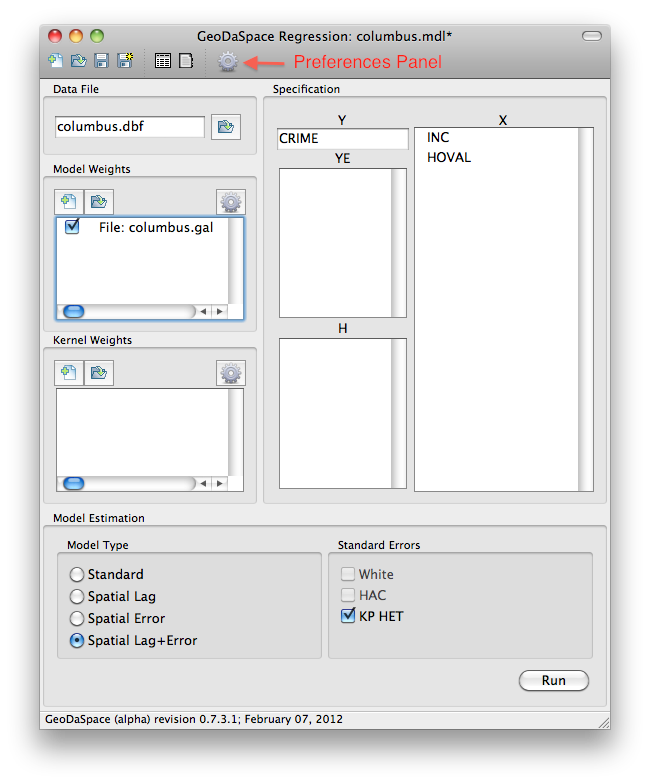
\includegraphics[width=0.7\textwidth]{GS_het_combo_pref.png}} \\
\subfloat[Preferences panel]{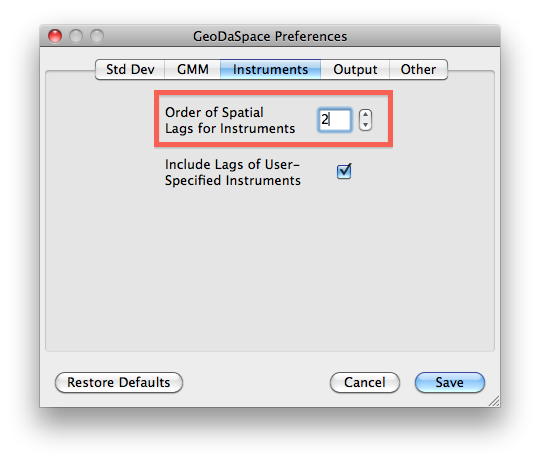
\includegraphics[width=0.7\textwidth]{GS_pref_lag.png}} \\
\end{figure}

Figure \ref{f:GS_het_endog} shows how to estimate spatial error models with endogenous variables and heteroskedasticity in GeoDaSpace. If the model contains other type of endogenous variables, but not a spatial lag, the results from GeoDaSpace match those from Stata without the need of any change (Table \ref{t:res_het_endog}).  

\begin{table}[htpb]
\caption{Comparison of the results of spatial error models with endogenous variables and heteroskedasticity}
\label{t:res_het_endog}
\centering
\begin{small}
\begin{tabular}{l|cccc} \hline
\textbf{Variable}&\textbf{GeoDaSpace}&\textbf{Stata}&\textbf{sphet}&\textbf{PySAL}\\ \hline
CONSTANT&82.2068&82.2068&&82.2068\\
&(15.2485)&(15.2485)&()&(15.2485)\\
INC&0.5785&0.5785&&0.5785\\
&(1.5024)&(1.5024)&()&(1.5024)\\
HOVAL&-1.4374&-1.4374&&-1.4374\\
&(0.9514)&(0.9514)&()&(0.9514)\\
lambda&0.4189&0.4189&&0.4189\\
&(0.1869)&(0.1869)&()&(0.1869)\\
\hline
\end{tabular}
\end{small}
\end{table}


\begin{figure}[htb]
\caption{Estimation of spatial error models with heteroskedasticity and endogenous variables using GeoDaSpace}
\label{f:GS_het_endog}
\begin{center}
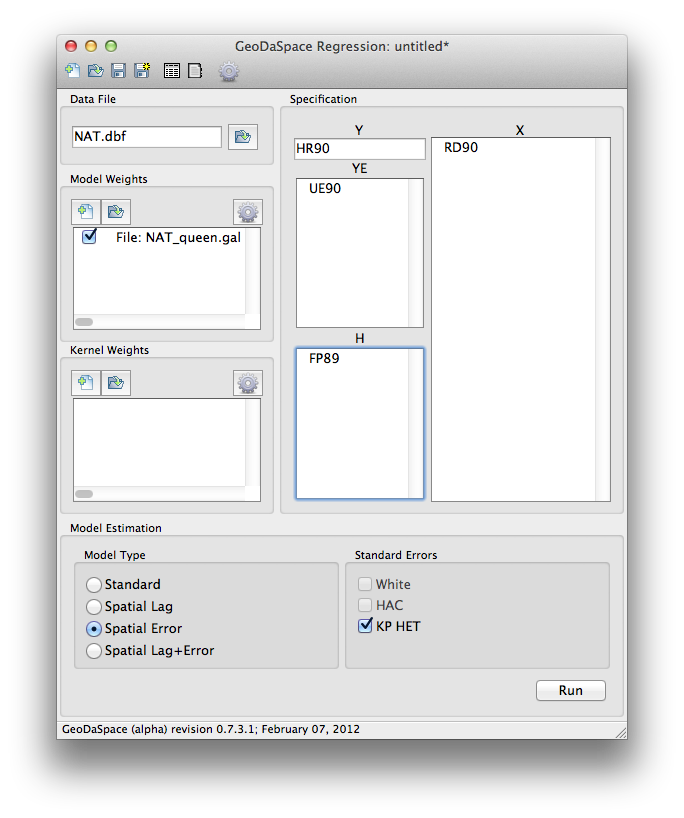
\includegraphics[width=0.7\linewidth]{GS_het_endog.png}\\
%\scriptsize{}
\end{center}
\end{figure}


In PySAL, these models could be estimated using the code shown in Listing \ref{lt:het_endog_stata}. This code is a continuation of Listing \ref{lt:het_stata}.

\begin{code}
\begin{lstlisting}[label=lt:het_endog_stata,caption=Using PySAL to match the results of spatial error models with heteroskedasticity and endogenous variables or spatial lag from Stata,language=Python]

#Spatial error model with spatial lag and
#    heteroskedasticity:
model = pysal.spreg.GM_Combo_Het(hr90,
        np.hstack((rd90,ue90)), w=w, w_lags=2)
print model.summary

#Adding instrument 'FP89':
fp89 = np.array([db.by_col('FP89')]).T

#Spatial error model with UE90 as endogenous variable
    and heteroskedasticity:
model = pysal.spreg.GM_Endog_Error_Het(hr90, rd90,
        yend=ue90, q=fp89, w=w)
print model.summary

\end{lstlisting}
\end{code}

\subsection{Step1c}
\label{s:step1c}
In addition to the number of lags of the exogenouns variables to be used as instruments, both GeoDaSpace and PySAL also offer the possibility to add the Step 1c in the estimation of the model as proposed by \citet{Arraiz10}. Step 1c updates the initial consistent estimation of lambda using a weighted nonlinear least squares solution to the moments equations. This results in a consistent and efficient intermediate estimation of lambda. Note however that a consistent estimation at this stage is already sufficient to obtain a consistent estimation of all parameters in the model. The option to run Step 1c can be found in the preferences panel in GeoDaSpace, as shown in Figure \ref{f:GS_pref_step1c}. In PySAL, all we have to do to select this option is add `step1c=True' to the arguments of the model.



\begin{figure}[htb]
\caption{Option to run Step1c from \citet{Arraiz10} for estimating spatial error models with heteroskedasticity using GeoDaSpace}
\label{f:GS_pref_step1c}
\begin{center}
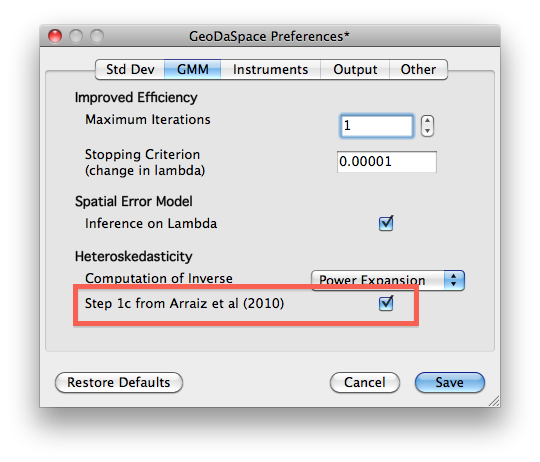
\includegraphics[width=0.7\linewidth]{GS_pref_step1c.png}\\
%\scriptsize{}
\end{center}
\end{figure}

\begin{code}
\begin{lstlisting}[label=lt:het_endog_stata,caption=Using PySAL to match the results of spatial error models with heteroskedasticity and endogenous variables or spatial lag from Stata,language=Python]

#Spatial error model with heteroskedasticity
#    (running Step1c):
model = pysal.spreg.GM_Error_Het(hr90,
        np.hstack((rd90,ue90)), w=w, step1c=True)
print model.summary

#Spatial error model with spatial lag and
    heteroskedasticity (running Step1c):
model = pysal.spreg.GM_Combo_Het(hr90,
        np.hstack((rd90,ue90)), w=w, step1c=True)
print model.summary

#Spatial error model with HOVAL as endogenous variable
    and heteroskedasticity (running Step1c):
model = pysal.spreg.GM_Endog_Error_Het(hr90, rd90,
        yend=ue90, q=fp89, w=w, step1c=True)
print model.summary

\end{lstlisting}
\end{code}


\newpage
\bibliography{bib}
\bibliographystyle{apalike}
\end{document}


